\documentclass[10pt]{beamer}

\usepackage{appendixnumberbeamer}
\usepackage{subcaption}
\usepackage{booktabs}
\usepackage[scale=2]{ccicons}

\usepackage{pgfplots}
\usepgfplotslibrary{dateplot}

\usepackage{xspace}

\title{Linear Programming Approach to the Graph Square Problem}
\date{
    \vspace{2em}
    Supervisor: Dr Christopher Duffy \\[1em]
    \today
} 
\author{Edward Xu}
\institute{University of Melbourne}

\begin{document}

\begin{frame}
  \maketitle
\end{frame}

\section[Intro]{Introduction}

\begin{frame}{Square of a Graph}
  \begin{figure}
    \centering
    \begin{subfigure}{0.34\textwidth}
      \centering
      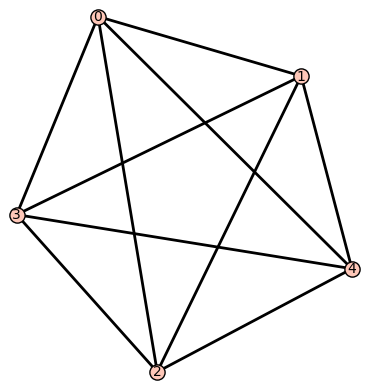
\includegraphics[width=\linewidth,height=0.42\textheight,keepaspectratio]{images/K5.png}
      \caption{$K_5$.}
      \label{fig:K5}
    \end{subfigure}
    \hfill
    \begin{subfigure}{0.34\textwidth}
      \centering
      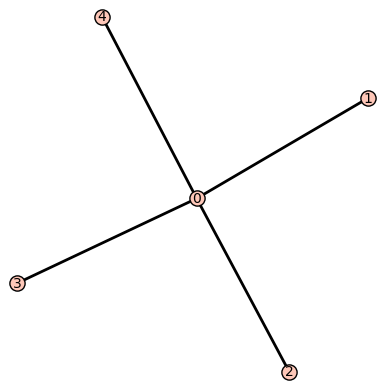
\includegraphics[width=\linewidth,height=0.42\textheight,keepaspectratio]{images/K5_root_11.png}
      \caption{$K_{1,4}$, a root of $K_5$.}
      \label{fig:K5_root}
    \end{subfigure}
    \caption{One of the $15$ non-isomorphic graph roots of $K_5$.}
    \label{fig:K5_example}
  \end{figure}
\end{frame}

\begin{frame}{The Graph Square Problem}

\end{frame}

\begin{frame}{Restricting on the Square vs the Root}

\end{frame}

\section[Algorithmic Approaches]{Algorithmic Approaches}

\begin{frame}{NP-Completeness}

\end{frame}

\begin{frame}{Maximal Cliques and Unicliqual Vertices in Tree Roots}

\end{frame}

\begin{frame}{Integer Program}

\end{frame}

\section[Square of a Tree]{Square of a Tree}

\begin{frame}{Linear Relaxation}

\end{frame}

\begin{frame}{Min and Max Objective Function}

\end{frame}

\begin{frame}{Identifying Square Characteristics of Tree Roots}

\end{frame}

\begin{frame}{Leaf Fixing Linear Program}

\end{frame}

\begin{frame}{Propagation of the Fixing}

\end{frame}

\section[Further Work]{Further Work}

\begin{frame}{Vertex Deletion}

\end{frame}

\begin{frame}{Symbolic Sets}

\end{frame}

\begin{frame}{Duality}

\end{frame}

\end{document}